\documentclass[12pt]{article}
\usepackage[margin=1in]{geometry}
\usepackage{graphicx}
\usepackage{booktabs}
\usepackage{xcolor}
\usepackage{float}
\usepackage{hyperref}
\usepackage{amsmath}
\usepackage{setspace}

\hypersetup{
    colorlinks=true,
    linkcolor=blue!60!black,
    citecolor=blue!60!black,
    urlcolor=blue!60!black
}
\onehalfspacing

\title{
    \vspace{-1cm}
    \large\textbf{Marketing A/B Testing Analysis:\\
    The Effect of Advertisement on Customer Conversion Rate}
}
\author{
    William Chen
}
\date{}

\setlength{\parindent}{0pt}
\setlength{\parskip}{8pt}

\begin{document}

\maketitle
\thispagestyle{empty}

\begin{abstract}
This report presents an A/B testing analysis of a digital marketing campaign, 
examining whether exposure to a commercial advertisement (\textit{ad}) increases 
conversion rate compared to a public service announcement (\textit{psa}) across 
588,101 users. Both Frequentist and Bayesian approaches are applied to a binary 
conversion outcome (\textit{converted}) and subgroup analyses by day and hour of 
peak ad exposure.

Frequentist results show a statistically significant difference in conversion rate 
($\chi^2(1) = 54.006$, $p < 0.001$), with the \textit{ad} group achieving 2.55\% 
compared to 1.79\% for \textit{psa}. Bayesian posterior analysis confirms a 
100\% probability that \textit{ad} yields a higher conversion rate, with an 
estimated advantage of 0.59\%--0.94\%. Subgroup analysis identifies Monday and 
the afternoon hours (14:00--20:00) as the highest-performing conditions. All 
effect sizes remain negligible, though the consistency across both methods 
supports the effectiveness of commercial advertisement exposure.
\end{abstract}

\newpage

% ══════════════════════════════════════════════════════════
\section{Introduction}
% ══════════════════════════════════════════════════════════
Understanding the effectiveness of digital advertisement is critical for 
optimizing marketing strategies and maximizing return on investment. While 
traditional metrics such as click-through rates provide surface-level insights, 
conversion rate, the proportion of users who complete a purchase after exposure, 
serves as a more direct measure of advertisement effectiveness.

This report presents an A/B testing analysis of a digital marketing campaign, 
examining whether exposure to a commercial advertisement (\textit{ad}) leads to 
a higher conversion rate compared to a public service announcement (\textit{psa}). 
The dataset contains 588,101 user records, with users randomly assigned to one 
of two experimental groups.

Both Frequentist and Bayesian approaches are applied to evaluate the primary 
binary outcome (\textit{converted}) and to examine conversion patterns across 
days and hours of peak ad exposure. The Frequentist approach determines whether 
observed differences are statistically significant, while the Bayesian approach 
provides posterior probabilities and credible intervals for a more interpretable 
conclusion.

% ══════════════════════════════════════════════════════════
\section{Data}
% ══════════════════════════════════════════════════════════

\subsection{Dataset Overview}

The dataset contains 588,101 user records sourced from Kaggle, collected from 
a randomized A/B experiment conducted on a digital marketing campaign. Users were 
randomly assigned to one of two experimental groups: \textit{psa} (control, 
$n = 23{,}524$) and \textit{ad} (treatment, $n = 564{,}577$). No missing values 
were detected across all variables. The primary outcome variable is 
\textit{converted}, a binary indicator representing whether a user made a purchase 
after being exposed to the advertisement.

\subsection{Feature Description}

The dataset contains 6 variables: 1 identifier (\textit{user.id}, excluded from 
analysis), 1 grouping variable (\textit{test.group}), 1 behavioral metric 
(\textit{total.ads}), 1 binary outcome variable (\textit{converted}), and 2 
temporal variables (\textit{most.ads.day}, \textit{most.ads.hour}). 
\textit{test.group} indicates the experimental group assigned to each user, either 
\textit{psa} (control) or \textit{ad} (treatment). \textit{total.ads} records the 
total number of advertisements viewed by each user. \textit{converted} is a logical 
variable indicating whether a user completed a purchase. \textit{most.ads.day} and 
\textit{most.ads.hour} record the day of the week and hour of the day during which 
the user was most frequently exposed to advertisements, respectively.

% ══════════════════════════════════════════════════════════
\section{Exploratory Data Analysis}
% ══════════════════════════════════════════════════════════

\subsection{Summary Statistics}

The dataset contains 588,101 complete observations with no missing values detected.
The two experimental groups are imbalanced by design: \textit{psa} contains 23,524 
users (4.0\%) and \textit{ad} contains 564,577 users (96.0\%). The overall 
conversion rate is 2.52\%, with \textit{ad} achieving 2.55\% and \textit{psa} 
achieving 1.79\%. \textit{total.ads} ranges from 1 to 2,065 with a mean of 24.82 
and a median of 13, indicating a heavily right-skewed distribution.

\subsection{Conversion Rate by Test Group}

Figure~\ref{fig:conversion_rate_bar} shows the conversion rates for both experimental 
groups. The \textit{ad} group achieves a higher conversion rate (2.55\%) compared to 
the \textit{psa} group (1.79\%), indicating a descriptive difference of 0.76 
percentage points. Whether this difference is statistically significant is examined 
in the Results section.

\begin{figure}[H]
    \centering
    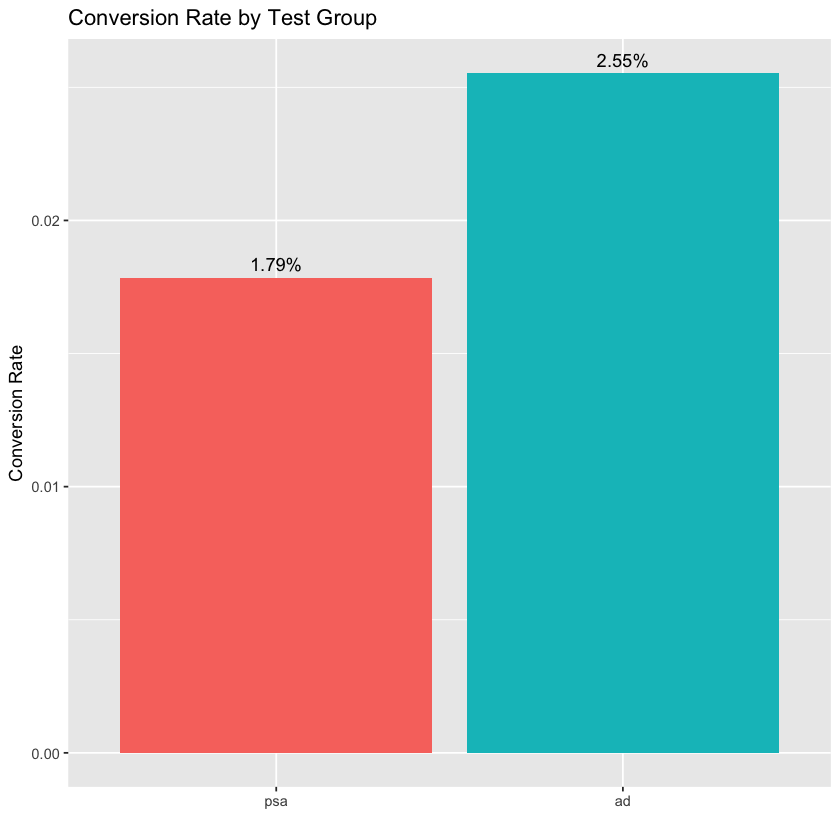
\includegraphics[width=0.55\textwidth]{figures/conversion_rate_bar.png}
    \caption{Conversion Rate by Test Group}
    \label{fig:conversion_rate_bar}
\end{figure}

\subsection{Conversion Rate by Day and Hour}

As shown in Figure~\ref{fig:conversion_day}, Monday consistently shows the highest 
conversion rate in the \textit{ad} group, while Thursday, Friday, and Saturday 
perform lower. Figure~\ref{fig:conversion_hour} shows that the afternoon period 
(14:00--20:00) achieves the highest conversion rates, with hour 16 reaching the peak.

\begin{figure}[H]
    \centering
    \begin{minipage}{0.48\textwidth}
        \centering
        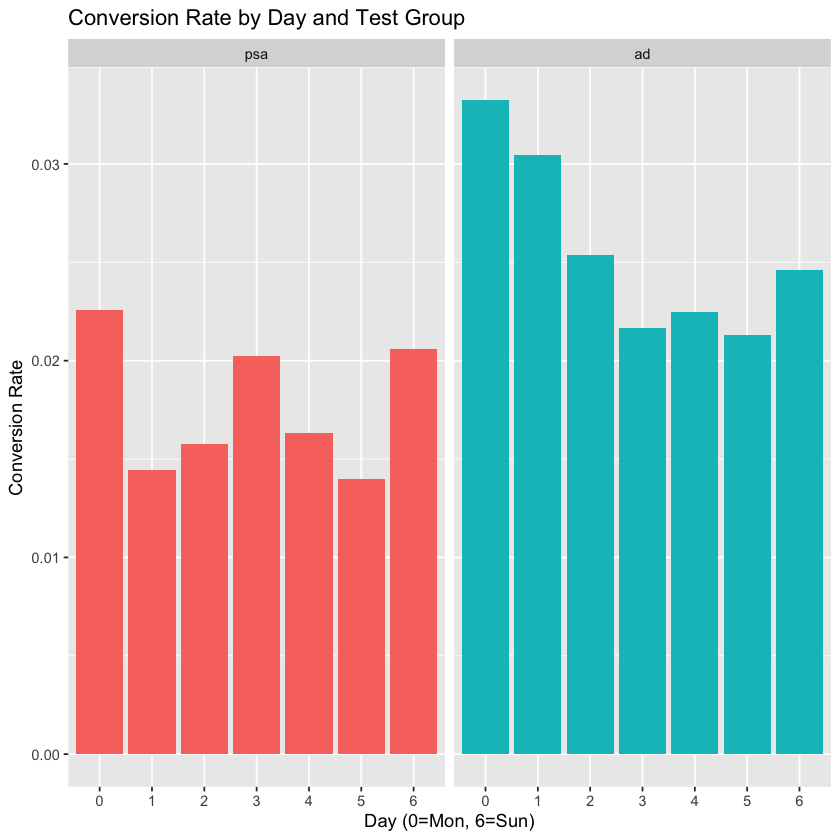
\includegraphics[width=\textwidth]{figures/conversion_rate_by_day.png}
        \caption{Conversion Rate by Day}
        \label{fig:conversion_day}
    \end{minipage}
    \hfill
    \begin{minipage}{0.48\textwidth}
        \centering
        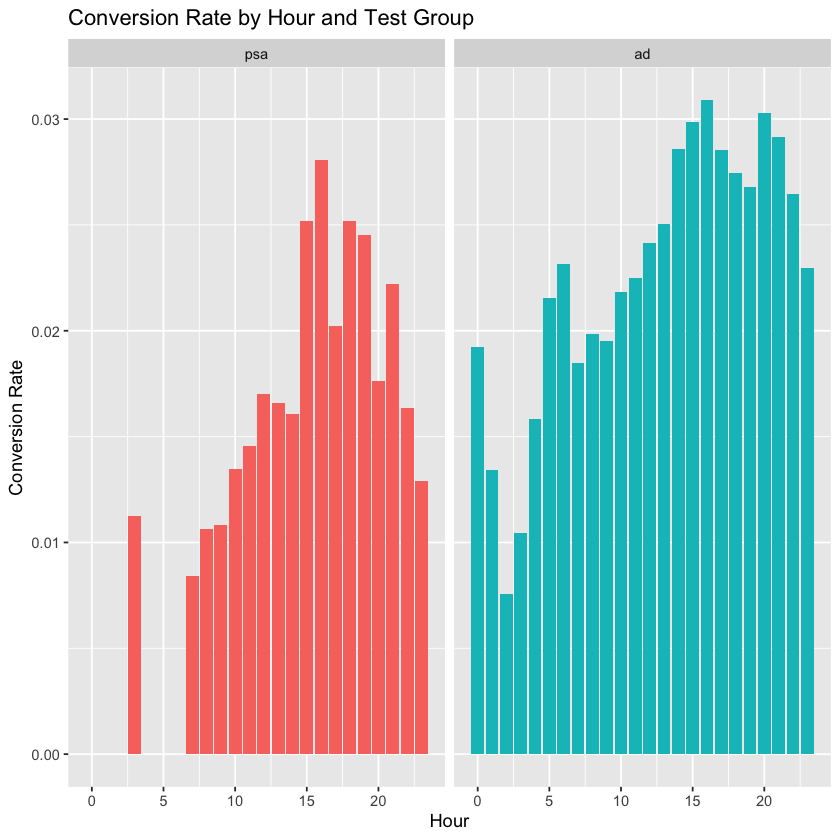
\includegraphics[width=\textwidth]{figures/conversion_rate_by_hour.png}
        \caption{Conversion Rate by Hour}
        \label{fig:conversion_hour}
    \end{minipage}
\end{figure}

Figure~\ref{fig:heatmap_conversion} and Figure~\ref{fig:heatmap_sample} present 
the conversion rate and sample size heatmaps for the \textit{ad} group. The 
notably high conversion rate observed on Saturday during early morning hours 
corresponds to cells with substantially fewer observations. In low-sample cells, 
a small number of conversions can produce a large rate spike, making such estimates 
unreliable. Elevated rates in these periods are therefore more likely to reflect 
random fluctuation than genuine user behavior.

\begin{figure}[H]
    \centering
    \begin{minipage}{0.45\textwidth}
        \centering
        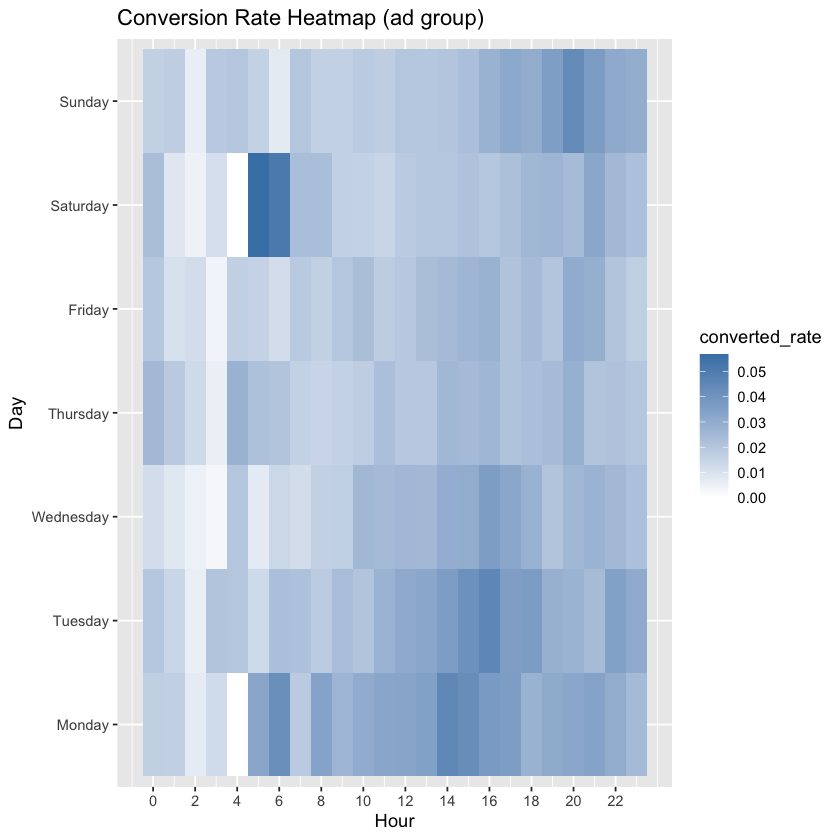
\includegraphics[width=\textwidth]{figures/heatmap_conversion.png}
        \caption{Conversion Rate Heatmap (ad group)}
        \label{fig:heatmap_conversion}
    \end{minipage}
    \hfill
    \begin{minipage}{0.45\textwidth}
        \centering
        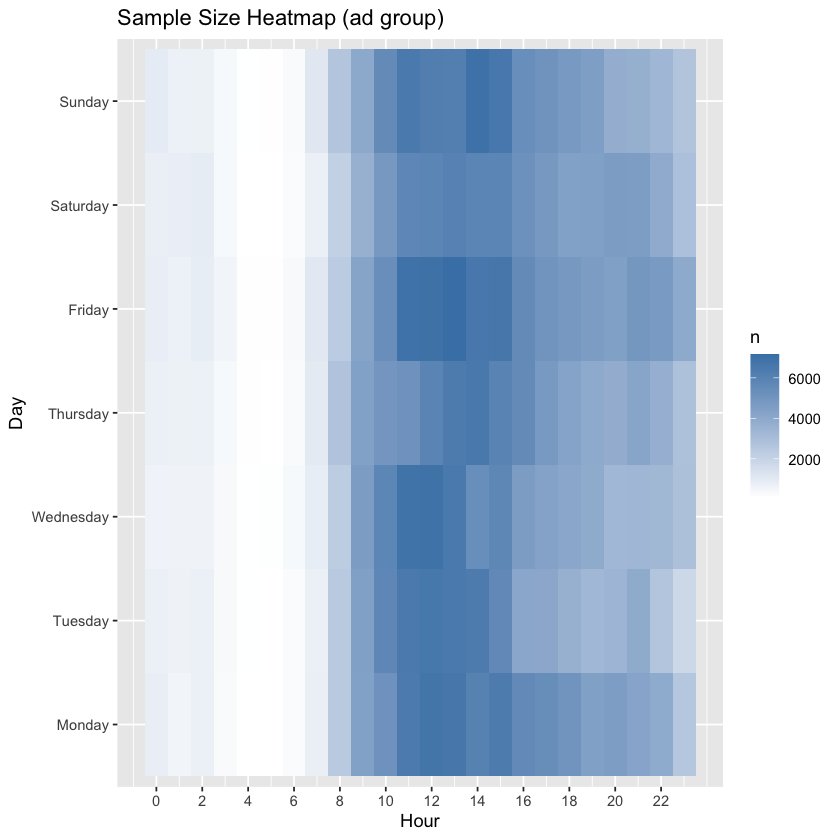
\includegraphics[width=\textwidth]{figures/heatmap_sample_size.png}
        \caption{Sample Size Heatmap (ad group)}
        \label{fig:heatmap_sample}
    \end{minipage}
\end{figure}

\subsection{Outlier Detection}

To assess the presence of extreme values in \textit{total.ads}, the IQR method 
was applied with a threshold of IQR $\times$ 3. The upper bound was determined 
to be 96, with 24,825 observations (4.22\%) exceeding this threshold. 
Figure~\ref{fig:outlier_boxplot} visualizes the outlier threshold across both 
groups on a log scale.

Users exceeding the upper bound exhibit substantially higher conversion rates 
(17.18\% for \textit{ad}, 11.51\% for \textit{psa}) compared to non-outlier 
users (1.91\% and 1.31\%, respectively), suggesting that high ad exposure is 
associated with increased conversion likelihood. As these represent genuine 
high-engagement users rather than data errors, outliers are retained in the 
analysis.

\begin{figure}[H]
    \centering
    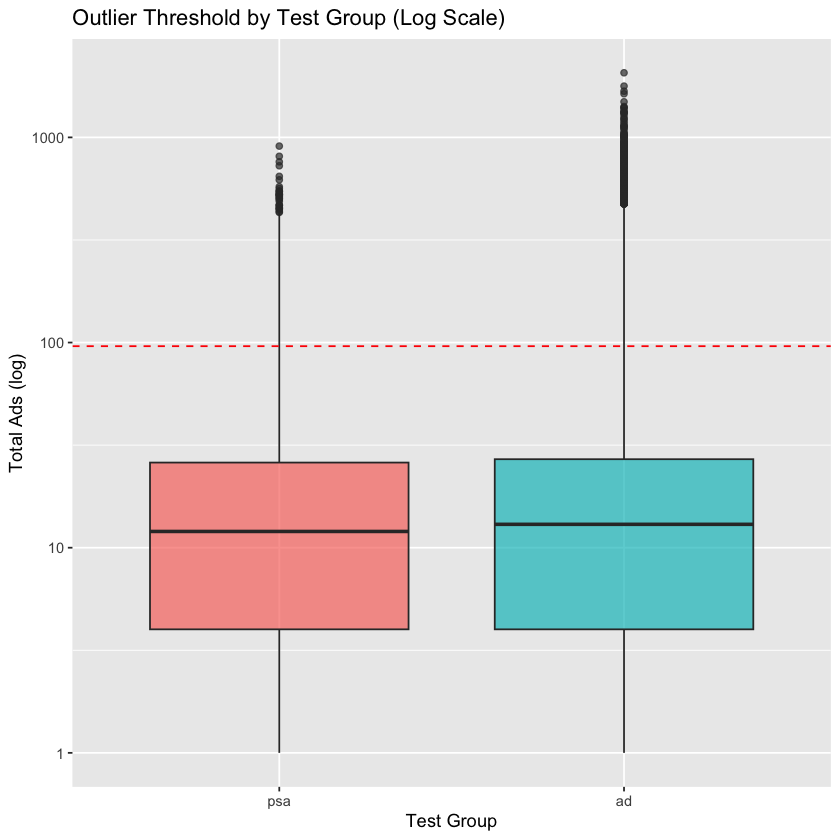
\includegraphics[width=0.6\textwidth]{figures/total_ads_boxplot.png}
    \caption{Total Ads Distribution by Group (Log Scale). The dashed red line 
    indicates the IQR $\times$ 3 outlier threshold.}
    \label{fig:outlier_boxplot}
\end{figure}

% TODO

% ══════════════════════════════════════════════════════════
\section{Methodology}
% ══════════════════════════════════════════════════════════

\subsection{Frequentist Approach}

\paragraph{Mann-Whitney U Test}
The Mann-Whitney U test was applied to compare \textit{total.ads} between the two 
groups. As a non-parametric test, it does not assume normality and is therefore 
appropriate for the right-skewed distribution of ad exposure counts.

\paragraph{Two-Sample Proportion Test}
The two-sample proportion test was applied to evaluate whether advertisement exposure 
is associated with a higher conversion rate. The null hypothesis states that the 
conversion rate is independent of group assignment.

\paragraph{Chi-Square Test}
The Chi-square test of independence was applied to evaluate whether conversion rate 
varies across days and hours within the \textit{ad} group.


\subsection{Bayesian Approach}

\paragraph{Beta-Binomial Model}
For binary conversion outcomes, a Beta-Binomial conjugate model was applied with 
an uninformative prior $\text{Beta}(1, 1)$, yielding the posterior:
\[
p \mid \text{data} \sim \text{Beta}(\alpha + \text{successes},\ \beta + \text{failures})
\]

\paragraph{Gamma-Poisson Model}
For \textit{total.ads}, a Gamma-Poisson conjugate model was applied with 
prior $\text{Gamma}(1, 1)$, yielding the posterior:
\[
\lambda \mid \text{data} \sim \text{Gamma}\!\left(\alpha + \sum x_i,\ \beta + n\right)
\]

\subsection{Evaluation Metrics}

\paragraph{Frequentist}
Frequentist tests are evaluated using p-value and effect size: Cohen's $h$ for 
the two-sample proportion test, Cramér's $V$ for Chi-square tests, and 
rank-biserial $r$ for the Mann-Whitney U test.

\paragraph{Bayesian}
For Bayesian models, Monte Carlo sampling ($n = 100{,}000$) was used to estimate 
the following metrics:

\begin{itemize}
    \item $P(\textit{ad} > \textit{psa})$: posterior probability that \textit{ad} 
    outperforms \textit{psa}
    \item \textbf{95\% HDI}: the Highest Density Interval representing the most 
    credible range of the difference between groups
\end{itemize}


% ══════════════════════════════════════════════════════════

\section{Frequentist Results}
% ══════════════════════════════════════════════════════════

\subsection{Primary Analysis (converted)}

A randomization check confirms that the two groups received comparable ad exposure 
(mean: 24.76 vs.\ 24.82), with no meaningful difference detected by the Mann-Whitney 
U test ($r = 0.0086$, small), supporting the validity of the experimental design.

The two-sample proportion test reveals a statistically significant difference in 
conversion rate between the \textit{ad} and \textit{psa} groups ($\chi^2(1) = 54.006$, 
$p < 0.001$). The \textit{ad} group achieves a conversion rate of 2.55\%, compared 
to 1.79\% for \textit{psa}, yielding a difference of 0.76 percentage points 
(95\% CI: $[-0.0095, -0.0059]$). However, Cohen's $h = 0.053$ indicates a negligible 
practical effect size.

\begin{figure}[H]
    \centering
    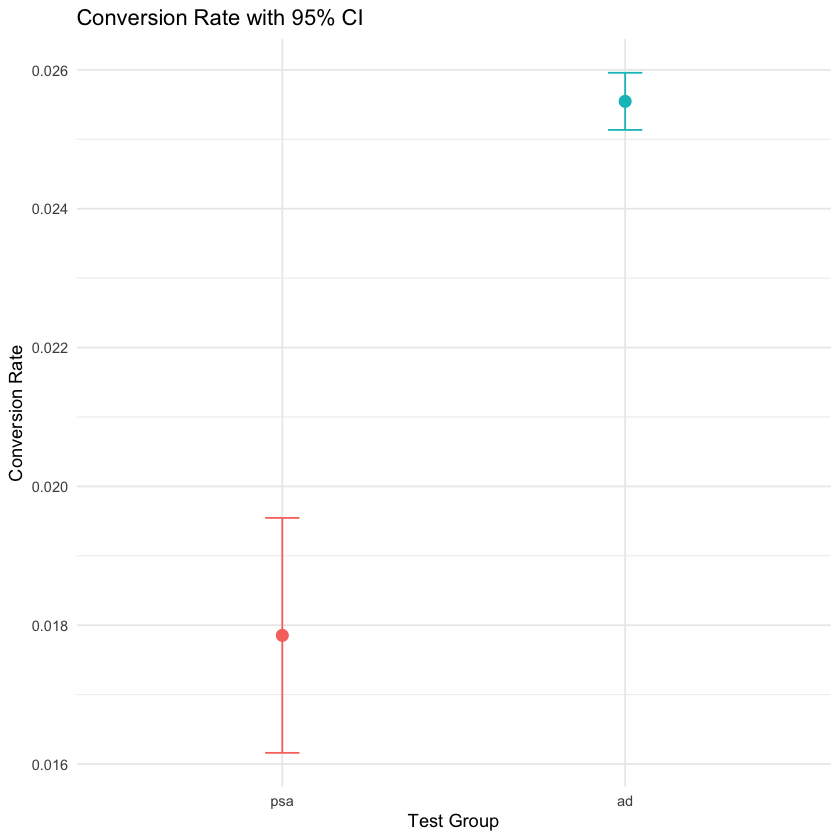
\includegraphics[width=0.55\textwidth]{figures/conversion_rate_ci.png}
    \caption{Conversion Rate with 95\% CI by Test Group}
    \label{fig:conversion_rate_ci}
\end{figure}

\subsection{Subgroup Analysis (ad group only)}

To further examine the conditions under which advertisement exposure is most 
effective, conversion rates within the \textit{ad} group are analyzed by day 
and hour of peak ad exposure. Table~\ref{tab:day_summary} presents the conversion 
rates by day. Monday achieves the highest conversion rate (3.32\%) with the largest 
positive residual ($+13.92$), while Saturday records the lowest (2.13\%, residual 
$= -7.45$).

The Chi-square test confirms a significant difference across days 
($\chi^2(6) = 412.79$, $p < 0.001$, Cramér's $V = 0.027$), and pairwise tests with 
Bonferroni correction show that Monday differs significantly from all other days 
($p \leq 0.034$), while Thursday, Friday, and Saturday show no significant 
differences among themselves ($p = 1.000$). Although statistically significant, 
Cramér's $V = 0.027$ indicates a negligible practical effect, suggesting that the 
difference in conversion rates across days is minimal in absolute terms (ranging 
from 2.13\% to 3.32\%).

\begin{table}[H]
\centering
\begin{tabular}{lrrr}
\toprule
\multicolumn{4}{l}{\textbf{Conversion Rate by Day (ad group)}} \\
\midrule
\textbf{Day} & \textbf{n} & \textbf{Conversion Rate} & \textbf{Std. Residual (TRUE)} \\
\midrule
Monday    & 83,571 & 3.32\% & $+13.92$ \\
Tuesday   & 74,572 & 3.04\% & $+8.36$  \\
Wednesday & 77,418 & 2.54\% & $-0.33$  \\
Thursday  & 79,077 & 2.16\% & $-6.88$  \\
Friday    & 88,805 & 2.25\% & $-5.75$  \\
Saturday  & 78,802 & 2.13\% & $-7.45$  \\
Sunday    & 82,332 & 2.46\% & $-1.66$  \\
\bottomrule
\end{tabular}
\caption{Conversion Rate and Standardized Residuals by Day (ad group)}
\label{tab:day_summary}
\end{table}

Table~\ref{tab:hour_summary} presents the conversion rates by hour within the 
\textit{ad} group, focusing on the top 10 performing hours (13:00--22:00). 
Hour 16 achieves the highest conversion rate (3.09\%, residual $= +6.34$), 
while hour 13 records the lowest (2.51\%, residual $= -0.64$), a difference 
of 0.58 percentage points.

The Chi-square test confirms a significant difference across hours 
($\chi^2(23) = 403.33$, $p < 0.001$, Cramér's $V = 0.0267$), and pairwise 
tests with Bonferroni correction show that hour 16 differs significantly from 
hour 13 ($p < 0.001$), while hours 14--20 form a non-significant cluster. 
Although statistically significant, Cramér's $V = 0.0267$ indicates a negligible 
practical effect, suggesting that the difference in conversion rates across hours 
is minimal in absolute terms.

\begin{table}[H]
\centering
\begin{tabular}{lrrr}
\toprule
\multicolumn{4}{l}{\textbf{Conversion Rate by Hour (ad group, Top 10)}} \\
\midrule
\textbf{Hour} & \textbf{n} & \textbf{Conversion Rate} & \textbf{Std. Residual (TRUE)} \\
\midrule
13 & 45,485 & 2.51\% & $-0.64$ \\
14 & 43,779 & 2.86\% & $+3.96$ \\
15 & 42,855 & 2.98\% & $+5.57$ \\
16 & 35,963 & 3.09\% & $+6.34$ \\
17 & 33,605 & 2.85\% & $+3.43$ \\
18 & 31,052 & 2.75\% & $+2.12$ \\
19 & 29,169 & 2.68\% & $+1.35$ \\
20 & 27,846 & 3.03\% & $+4.94$ \\
21 & 28,895 & 2.92\% & $+3.86$ \\
22 & 25,515 & 2.65\% & $+0.91$ \\
\bottomrule
\end{tabular}
\caption{Conversion Rate and Standardized Residuals by Hour, Top 10 (ad group)}
\label{tab:hour_summary}
\end{table}

\section{Bayesian Results}

A randomization check using the Gamma-Poisson model confirms that the two groups 
exhibit comparable ad exposure, with $P(\textit{ad} > \textit{psa}) = 97.19\%$ 
and a 95\% HDI of $[-0.0013, 0.1284]$ that includes zero, indicating no meaningful 
difference in \textit{total.ads} between groups. Figure~\ref{fig:posterior_total_ads} 
shows the posterior distributions of the average ad exposure rate for both groups.

\begin{figure}[H]
    \centering
    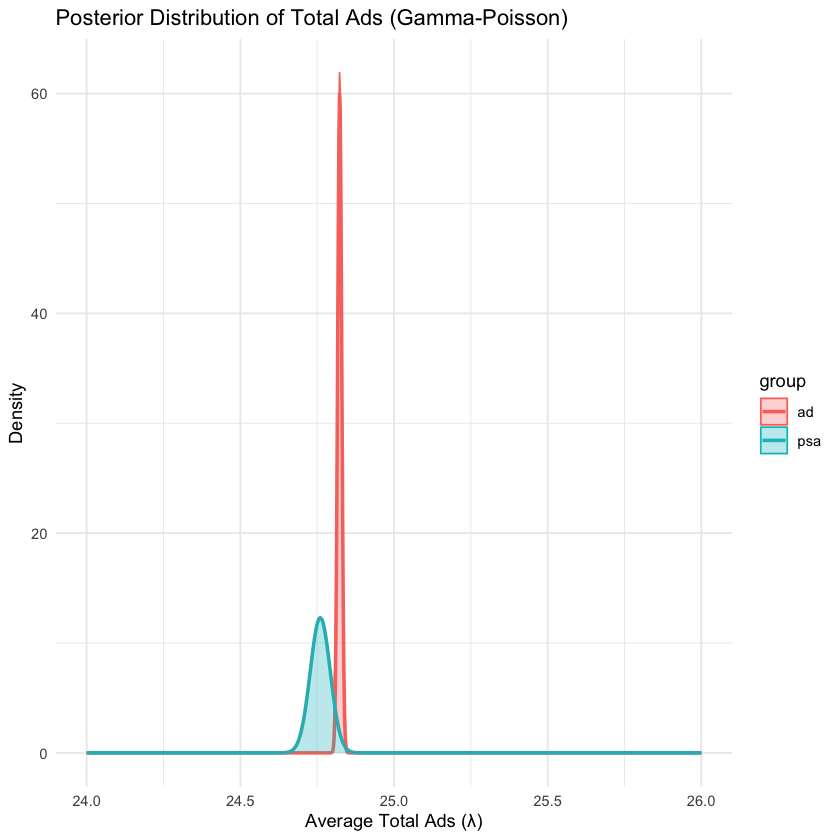
\includegraphics[width=0.6\textwidth]{figures/posterior_total_ads.png}
    \caption{Posterior Distribution of Total Ads Rate (Gamma-Poisson)}
    \label{fig:posterior_total_ads}
\end{figure}

\subsection{Primary Analysis (converted: Beta-Binomial)}

The Beta-Binomial model yields a posterior probability of $P(\textit{ad} > 
\textit{psa}) = 1.0000$, with a 95\% HDI of $[0.0059, 0.0094]$ that excludes 
zero, confirming that the \textit{ad} group achieves a higher conversion rate 
with near certainty. The posterior means are 2.55\% for \textit{ad} and 1.79\% 
for \textit{psa}. Figure~\ref{fig:posterior_converted} shows the posterior 
distributions of the conversion rate for both groups, with the \textit{ad} 
distribution shifted clearly to the right.

\begin{figure}[H]
    \centering
    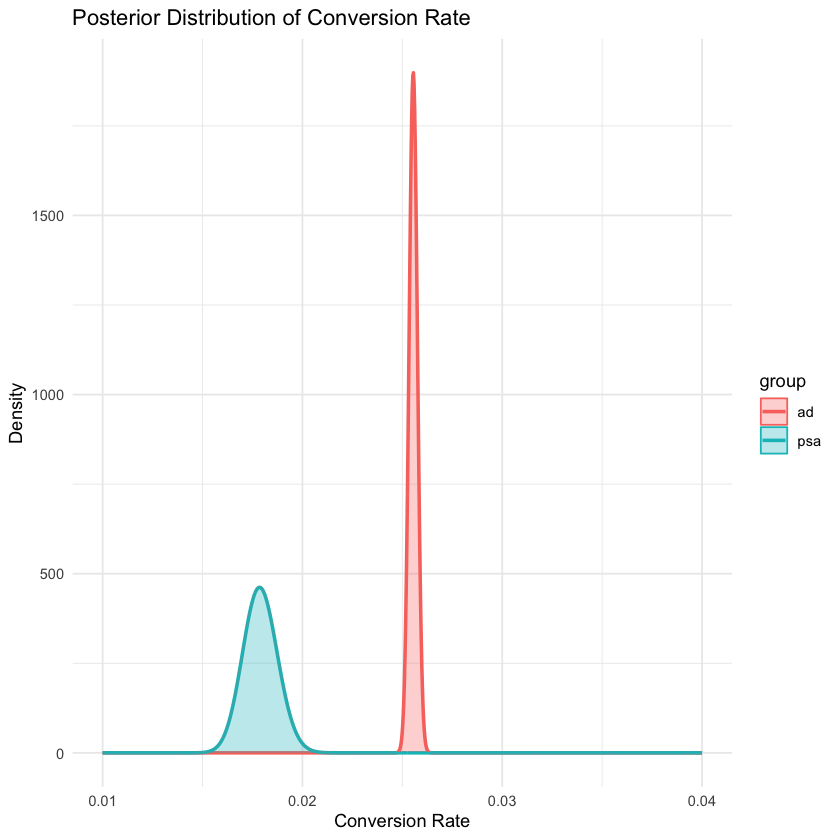
\includegraphics[width=0.6\textwidth]{figures/posterior_converted.png}
    \caption{Posterior Distribution of Conversion Rate (Beta-Binomial)}
    \label{fig:posterior_converted}
\end{figure}

\subsection{Subgroup Analysis (ad group only)}

Table~\ref{tab:bayes_day_summary} presents the posterior means and 95\% HDI of 
conversion rates by day within the \textit{ad} group. Monday achieves the highest 
posterior mean (3.33\%), while Saturday records the lowest (2.13\%). The 
non-overlapping HDIs between Monday and the lower-performing days confirm that 
the differences are credible rather than due to sampling variability.

Pairwise posterior comparisons show that Monday outperforms all other days with 
near certainty, including Tuesday ($P = 0.9993$, 95\% HDI: $[0.0011, 0.0045]$), 
while Thursday, Friday, and Saturday show no meaningful difference among themselves. 
Figure~\ref{fig:posterior_day} shows the posterior distributions for the three 
most contrasting days.

\begin{table}[H]
\centering
\begin{tabular}{lrrr}
\toprule
\multicolumn{4}{l}{\textbf{Posterior Conversion Rate by Day (ad group)}} \\
\midrule
\textbf{Day} & \textbf{Posterior Mean} & \textbf{HDI Lower} & \textbf{HDI Upper} \\
\midrule
Monday    & 3.33\% & 3.20\% & 3.45\% \\
Tuesday   & 3.05\% & 2.92\% & 3.17\% \\
Wednesday & 2.54\% & 2.43\% & 2.65\% \\
Thursday  & 2.17\% & 2.07\% & 2.27\% \\
Friday    & 2.25\% & 2.15\% & 2.34\% \\
Saturday  & 2.13\% & 2.03\% & 2.23\% \\
Sunday    & 2.46\% & 2.36\% & 2.57\% \\
\bottomrule
\end{tabular}
\caption{Posterior Conversion Rate by Day (ad group)}
\label{tab:bayes_day_summary}
\end{table}

\begin{figure}[H]
    \centering
    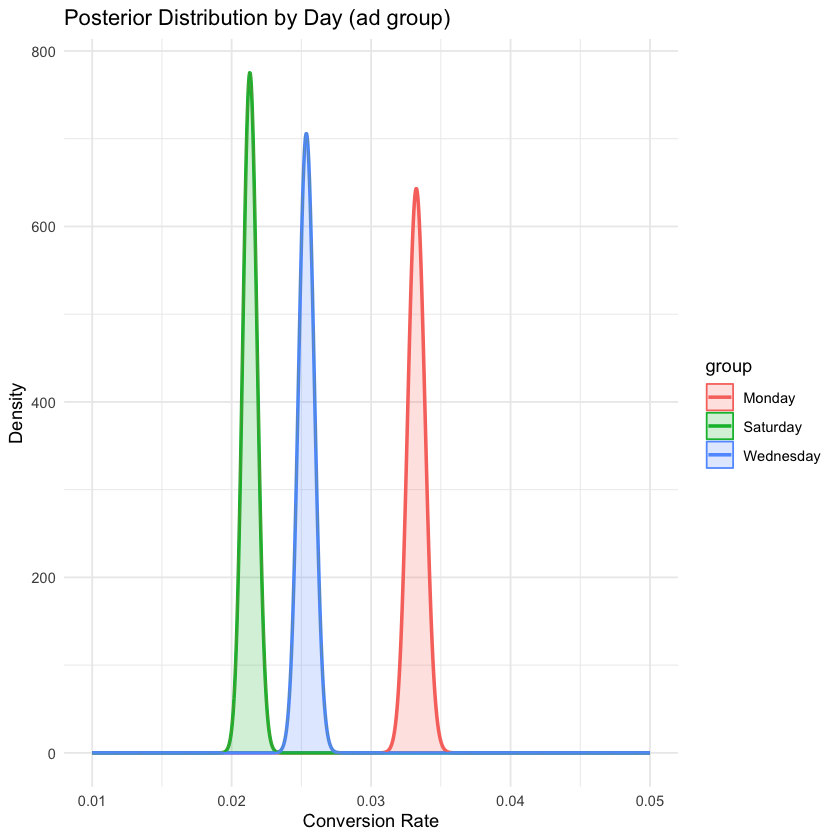
\includegraphics[width=0.6\textwidth]{figures/posterior_day.png}
    \caption{Posterior Distribution of Conversion Rate by Day (Monday, Wednesday, Saturday)}
    \label{fig:posterior_day}
\end{figure}

Table~\ref{tab:bayes_hour_summary} presents the posterior means and 95\% HDI of 
conversion rates by hour within the \textit{ad} group, focusing on the top 10 
performing hours (13:00--22:00). Hour 16 achieves the highest posterior mean 
(3.09\%), while hour 13 records the lowest (2.51\%).

Pairwise posterior comparisons show that hour 16 outperforms hour 13 with near 
certainty ($P = 1.0000$, 95\% HDI: $[0.0036, 0.0082]$), while hour 16 shows no 
meaningful difference from hours 15, 20, and 21 (HDI includes zero), suggesting 
that the afternoon peak (15:00--21:00) performs comparably.

\begin{table}[H]
\centering
\begin{tabular}{lrrr}
\toprule
\multicolumn{4}{l}{\textbf{Posterior Conversion Rate by Hour (ad group, Top 10)}} \\
\midrule
\textbf{Hour} & \textbf{Posterior Mean} & \textbf{HDI Lower} & \textbf{HDI Upper} \\
\midrule
13 & 2.51\% & 2.37\% & 2.65\% \\
14 & 2.86\% & 2.70\% & 3.02\% \\
15 & 2.99\% & 2.83\% & 3.15\% \\
16 & 3.09\% & 2.91\% & 3.27\% \\
17 & 2.86\% & 2.68\% & 3.04\% \\
18 & 2.75\% & 2.57\% & 2.93\% \\
19 & 2.68\% & 2.50\% & 2.87\% \\
20 & 3.03\% & 2.83\% & 3.23\% \\
21 & 2.92\% & 2.72\% & 3.11\% \\
22 & 2.65\% & 2.45\% & 2.85\% \\
\bottomrule
\end{tabular}
\caption{Posterior Conversion Rate by Hour, Top 10 (ad group)}
\label{tab:bayes_hour_summary}
\end{table}

\begin{figure}[H]
    \centering
    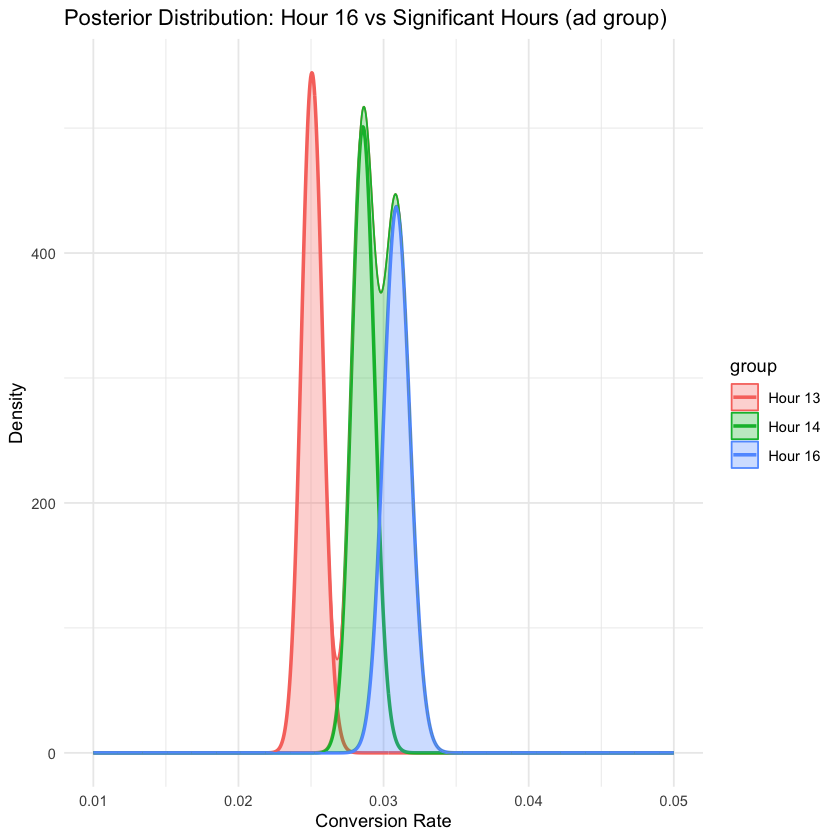
\includegraphics[width=0.6\textwidth]{figures/posterior_hour.png}
    \caption{Posterior Distribution of Conversion Rate by Hour (Hour 13, 14, 16)}
    \label{fig:posterior_hour}
\end{figure}


\section{Overall Comparison}

Both Frequentist and Bayesian approaches consistently confirm that advertisement 
exposure significantly increases conversion rate. The Frequentist two-sample 
proportion test yields $p < 0.001$, while the Bayesian Beta-Binomial model 
estimates $P(\textit{ad} > \textit{psa}) = 1.0000$ with a 95\% HDI of 
$[0.0059, 0.0094]$ excluding zero. However, both approaches agree that the 
practical effect is negligible (Cohen's $h = 0.053$).

For subgroup analysis, both approaches identify Monday and the afternoon hours 
(14:00--20:00) as the highest-performing conditions, with Hour 16 achieving the 
peak conversion rate. All effect sizes remain negligible, consistent with the 
large sample size inflating statistical significance.

% TODO

% ══════════════════════════════════════════════════════════
\section{Discussion \& Conclusion}
% ══════════════════════════════════════════════════════════

\subsection{Key Findings}

Both Frequentist and Bayesian analyses consistently confirm that advertisement 
exposure has a statistically significant positive effect on conversion rate. The 
\textit{ad} group achieves a conversion rate of 2.55\%, compared to 1.79\% for 
the \textit{psa} group, with near-certain posterior probability ($P = 1.0000$). 
Despite statistical significance, all effect sizes remain negligible, reflecting 
a common pattern in large-sample A/B tests where even trivial differences reach 
significance.

\subsection{Business Recommendations}

Based on the analysis, advertisement exposure is recommended to be prioritized 
on \textbf{Monday} and during \textbf{afternoon hours (14:00--20:00)}, 
particularly at \textbf{hour 16}, where conversion rates are consistently highest. 

Users with high ad exposure (\textit{total.ads} $> 96$) exhibit substantially 
higher conversion rates (17.18\%), suggesting that sustained advertisement 
exposure has a cumulative effect on purchase likelihood. Advertisers may therefore 
benefit from increasing ad frequency for engaged users rather than broadening 
reach to new audiences.

\subsection{Limitations}

\subsubsection*{Dataset Limitations}
The dataset does not include contextual variables such as user demographics, 
device type, or advertisement content, which may confound the relationship between 
ad exposure and conversion. Additionally, it is unclear whether \textit{total.ads} 
represents unique advertisement impressions or repeated exposures to the same 
advertisement, limiting the interpretability of the cumulative exposure effect.

\subsubsection*{Evaluation Metrics}
The analysis relies solely on \textit{converted} as the primary outcome metric. 
While conversion captures whether a purchase occurred, it does not reflect 
revenue per user or customer lifetime value, which would provide a more 
comprehensive evaluation of advertisement effectiveness. Furthermore, all effect 
sizes remain negligible despite statistical significance, suggesting that the 
practical impact of the findings should be interpreted with caution.
\begin{thebibliography}{9}

\bibitem{marketing}
% TODO

\end{thebibliography}

\end{document}